In this section of experiment, vee-belt is used and in order to determine the coefficient of friction $\mu$, we start varying the tension on the slack side $T_2$ and then find the corresponding tension on the tight side $T_1$ until the belt starts to slip while maintaining a constant angle of lap $\theta$ to be $40\degree$ and $\alpha$ of $38\degree$. The results of the experiments are shown on the table below.
\begin{table}[H]
\begin{center}
\begin{tabular}{c|c|c|}
\cline{2-3}
 & $M_2$ (kg)                                             & $M_1$(kg)   \\ \cline{2-3} 
 & 0.65$\pm$0.1                                            & 1.62$\pm$0.1 \\ \cline{2-3} 
 & \begin{tabular}[c]{@{}c@{}}1.16\\ ±0.1\end{tabular} & 2.25±0.1 \\ \cline{2-3} 
 & 1.66$\pm$0.1                                            & 3.05$\pm$0.1 \\ \cline{2-3} 
 & 2.16$\pm$0.1                                            & 4.05$\pm$0.1 \\ \cline{2-3} 
 & 2.66$\pm$0.1                                            & 5.17$\pm$0.1 \\ \cline{2-3} 
 & 3.17$\pm$0.1                                                & 6.42$\pm$0.1 \\ \cline{2-3} 
\end{tabular}
\caption{Vee belt friction experiment results.}
\label{tab: 9}
\end{center}
\end{table}

Multiplying the mass by the acceleration due to gravity and applying the same uncertainty equation as experiment above, then the tension for both the slack side and the tight side are given on the table below:
\begin{table}[H]
\begin{center}
\begin{tabular}{c|c|c|}
\cline{2-3}
 & $T_2$ (N)                                             & $T_1$(N)   \\ \cline{2-3} 
 & 6.37$\pm$0.98                                            & 15.9$\pm$0.98 \\ \cline{2-3} 
 & \begin{tabular}[c]{@{}c@{}}11.36$\pm$0.99\end{tabular} & 22.04$\pm$0.98 \\ \cline{2-3} 
 & 16.26$\pm$0.98                                            & 29.87$\pm$0.98 \\ \cline{2-3} 
 & 21.16$\pm$0.98                                            & 39.67$\pm$0.98 \\ \cline{2-3} 
 & 26.05$\pm$0.98                                            & 50.63$\pm$0.98 \\ \cline{2-3} 
 & 31.05$\pm$0.98                                                & 62.88$\pm$0.98\\ \cline{2-3} 
\end{tabular}
\caption{Tension of the vee belt.}
\label{tab: 10}
\end{center}
\end{table}

The graph of $T_2$ versus $T_1$ is shown below:
\begin{figure}[H]
\centering
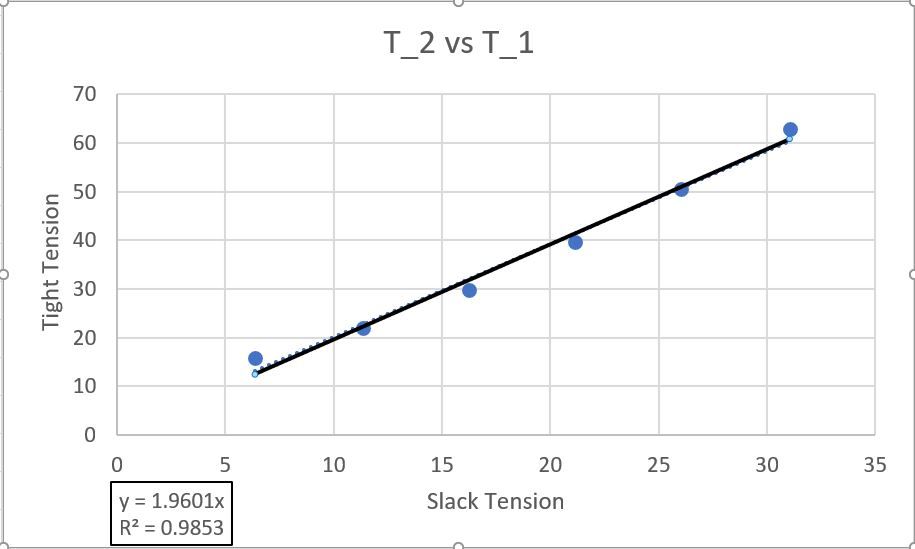
\includegraphics[width=1\textwidth]{chapters/lab2/m2}
\caption{$T_2$ versus $T_1$ graph.}
\label{fig:mesh3}
\end{figure}

The line of best fit of above graph has a gradient of 1.9601. To deduce $\mu$, we must calculate $\mu '$ first. Rearranging equation 6 to find $\mu '$, then $\mu'$ is given by:
\begin{align}
\mu ' &= \frac{1}{\theta}\ln\left(\frac{\delta T_1}{\delta T_2}\right) \notag
\end{align}
Where $\frac{\delta T_1}{\delta T_2}$ is equal to the gradient of the line of best fit above. Substituting all the required value into above equation, then $\mu '$ value to three significant figures calculated to be:
\begin{align}
\mu ' &= \frac{180}{40\pi}\ln\left(1.9601\right) \notag \\
\qquad &= 7.57\times10^{-1} \notag
\end{align}

Substituting the value of $\mu '$ and $\alpha$ into equation 7, then the $\mu$ to three significant is given by:
\begin{align}
\mu &= \mu ' * \cos(0.5\alpha) \notag \\
\qquad &= 0.757* \cos(0.5*\frac{38\pi}{180}) \notag \\
\qquad &=  0.716 \notag
\end{align}